\section{Indoor Positioning}
\subsection{Problem Statement}
Determining the user's precise starting position within an indoor environment is a critical first step for navigation. Unlike outdoor environments where GPS signals can be used reliably, indoor spaces lack such direct localization references. In expansive areas—where architectural features may be repetitive or ambiguous—automated recognition methods alone can struggle to identify the user's location uniquely. This challenge is compounded by the absence of distinct visual markers typically available in smaller, more controlled spaces.

\subsection{Solution}
\subsubsection{Auto Tracking for Small Area Targets}
For relatively small Area Targets, the positioning process can be fully automated. In these cases, the AR camera is designed to detect environmental features in real time and align them with the corresponding model data. This automatic alignment enables the system to accurately indicate the user's current position without requiring manual intervention.

As discussed in Section~\ref{subsub:AreaTargetObserver}, the tracking status is continuously monitored and updated. This information is then used to provide real-time feedback to the user, ensuring that necessary adjustments—such as reorienting the device or repositioning it slightly—can be made promptly to maintain optimal tracking performance.

Moreover, this automated approach simplifies the user experience in well-defined and controlled spaces. Since small Area Targets typically offer distinct and easily recognizable visual cues, the system can quickly and efficiently lock onto these features, resulting in a more stable and reliable positioning solution. However, it is essential to note that while auto-tracking is highly effective for small Area Targets, it may become less reliable when dealing with larger or multiple Area Targets, where environmental similarities (such as similar-looking floors) can cause ambiguities in target detection.

\subsubsection{Location Prior for Large Area Targets}\label{subsub:LocationPrior}
In environments featuring large or architecturally repetitive Area Targets, incorporating a location prior greatly enhances the localization process. A location prior provides direct guidance to the Area Target Observer, ensuring that targets are accurately aligned with their surrounding environment and improving the speed of the initial localization.

Location priors work by managing the loading of data from a set of activated Area Targets that have \texttt{requireExternalPositions} set to \texttt{VU\_TRUE}. The Vuforia Engine leverages this configuration to select and load the most relevant Area Targets based on both proximity and overlapping regions with the externally provided position. As a result, only the necessary target data is asynchronously loaded when an external position is set, which not only accelerates first-time localization but also minimizes tracking errors—particularly when the tracked position falls outside the intended region of an Area Target.

As a best practice, assigning an external prior for each large Area Target allows the Vuforia Engine to consistently choose the most appropriate and nearest targets among those activated. This is especially beneficial in scenarios where similar or repetitive features exist—such as different floors of the same building—ensuring a more reliable and efficient tracking experience.

\subsubsection{Positioning with QR Codes}
We implement a positioning system using QR Codes to provide accurate location tracking within a building. Predefined QR Codes are placed at pivotal positions, such as landings at the start of each new floor, to serve as location references. When users enter a floor or need to reposition after losing track of their environment, they can scan these QR Codes. The application will use the encoded position information as the location prior (as discussed in Section~\ref{subsub:LocationPrior}) to enhance relative positioning and tracking accuracy.

\subsubsubsection*{Generating QR Codes}
To encode positional data (x, y, z) into QR codes, we use Python's \texttt{qrcode} library. The following script generates a QR code containing JSON-formatted positional data:

\begin{lstlisting}[language=cSharp]
data = {"x": 1, "y": 2, "z": 3}
json_data = json.dumps(data)
qr = qrcode.QRCode(
    version=1,
    error_correction=qrcode.constants.ERROR_CORRECT_L,
    box_size=10,
    border=4,
)
qr.add_data(json_data)
qr.make(fit=True)

img = qr.make_image(fill='black', back_color='white')
img.save("qr_code.png")
\end{lstlisting}

This script generates a QR code containing the JSON-encoded coordinates of a location in the building.

\subsubsubsection*{Scanning QR Codes in Unity}
In Unity, we created a new scene that allows users to scan QR codes and extract encoded positional data. The scanning functionality is implemented using the \texttt{ZXing} library for barcode detection. Below are the key code segments and their detailed explanations.

\begin{itemize}
    \item \textbf{Defining the QRData Class}

    \begin{lstlisting}[style=cSharp]
    [Serializable]
    public class QRData
    {
        public int x;
        public int y;
        public int z;
    }
    \end{lstlisting}
    The \texttt{QRData} class is used to store positional data (x, y, z) extracted from the scanned QR code.

    \item \textbf{Variable Declarations and Camera Setup}
    \begin{lstlisting}[style=cSharp]
    [SerializeField] private RawImage _rawImageBackground;
    [SerializeField] private AspectRatioFitter _aspectRatioFitter;
    [SerializeField] private TextMeshProUGUI _textOut;
    [SerializeField] private RectTransform _scanZone;
    private bool _isCamAvailable;
    private WebCamTexture _cameraTexture;
    \end{lstlisting}
    These variables handle the camera feed and display the scanned QR code data on the UI.
    
    \begin{lstlisting}[style=cSharp]
    void Start()
        SetUpCamera();
    \end{lstlisting}
    When the scene starts, the \texttt{Start()} function calls \texttt{SetUpCamera()} to initialize the camera.

    \item \textbf{Setting Up the Camera for QR Scanning}
        \begin{lstlisting}[style=cSharp]
        private void SetUpCamera(){
            WebCamDevice[] devices = WebCamTexture.devices;
            if (devices.Length == 0){
                _isCamAvailable = false;
                return;
            }
            for (int i = 0; i < devices.Length; i++){
                if (!devices[i].isFrontFacing){
                    _cameraTexture = new WebCamTexture(devices[i].name, 
                        (int)_scanZone.rect.width, (int)_scanZone.rect.height);
                }
            }
            _cameraTexture.Play();
            _rawImageBackground.texture = _cameraTexture;
            _isCamAvailable = true;
        }
        \end{lstlisting}
        The \texttt{SetUpCamera()} function checks available camera devices, selects the back camera, and starts capturing video.

    \item \textbf{Updating the Camera Feed Display}
        \begin{lstlisting}[style=cSharp]
        private void UpdateCameraRender(){
            if (!_isCamAvailable){
                return;
            }
            float ratio = (float)_cameraTexture.width / (float)_cameraTexture.height;
            _aspectRatioFitter.aspectRatio = ratio;
            int orientation = -_cameraTexture.videoRotationAngle;
            _rawImageBackground.rectTransform.localEulerAngles = new Vector3(0, 0, orientation);
        }
        \end{lstlisting}
        This function adjusts the camera feed's aspect ratio and rotation to align with the screen display.

    \item \textbf{QR Code Scanning and Data Processing}
    \begin{lstlisting}[style=cSharp]
    public void OnClickScan()
        Scan();
    \end{lstlisting}
    The \texttt{OnClickScan()} function is triggered when the user presses the scan button.

    \begin{lstlisting}[style=cSharp]
    private void Scan(){
        try{
            IBarcodeReader barcodeReader = new BarcodeReader();
            Result result = barcodeReader.Decode(
                _cameraTexture.GetPixels32(), 
                _cameraTexture.width, 
                _cameraTexture.height
            );
    
            if (result != null){
                try{
                    QRData qrData = JsonUtility.FromJson<QRData>(result.Text);
                    _textOut.text = $"x: {qrData.x}, y: {qrData.y}, z: {qrData.z}";
                }
                catch{
                    _textOut.text = "INVALID QR CODE FORMAT";
                }
            }
            else{
                _textOut.text = "FAILED TO SCAN QRCODE";
            }
        }
        catch{
            _textOut.text = "FAILED IN TRY";
        }
    }
    \end{lstlisting}
    The \texttt{Scan()} function uses \texttt{ZXing} to decode the QR code from the camera feed. If a valid QR code is detected, it converts the JSON-formatted string into a \texttt{QRData} object and displays the extracted coordinates on the UI. An error message is shown if the QR code is invalid or scanning fails.

    \item \textbf{Summary}
        \begin{itemize}
            \item \textbf{Camera Setup}: Retrieves available devices, selects the back camera, and starts video capture.
            \item \textbf{Camera Feed Update}: Adjusts the display aspect ratio and orientation.
            \item \textbf{QR Code Scanning}: Reads the QR code, verifies the format, and displays the decoded data.
        \end{itemize}
\end{itemize}

\subsubsubsection*{Integration in the Application}
When a user scans a QR code, the application extracts the encoded coordinates and uses them as the new reference position. This functionality ensures accurate indoor navigation, improving tracking performance in augmented reality applications using Vuforia Engine. After scanning a QR code, the application automatically starts a new tracking session, ensuring precise localization within the defined model area. In addition, 

This implementation provides a robust and scalable approach to positioning using QR codes, combining Python for QR code generation and Unity with ZXing for QR code scanning and interpretation.

\begin{figure}[ht]
  \centering
  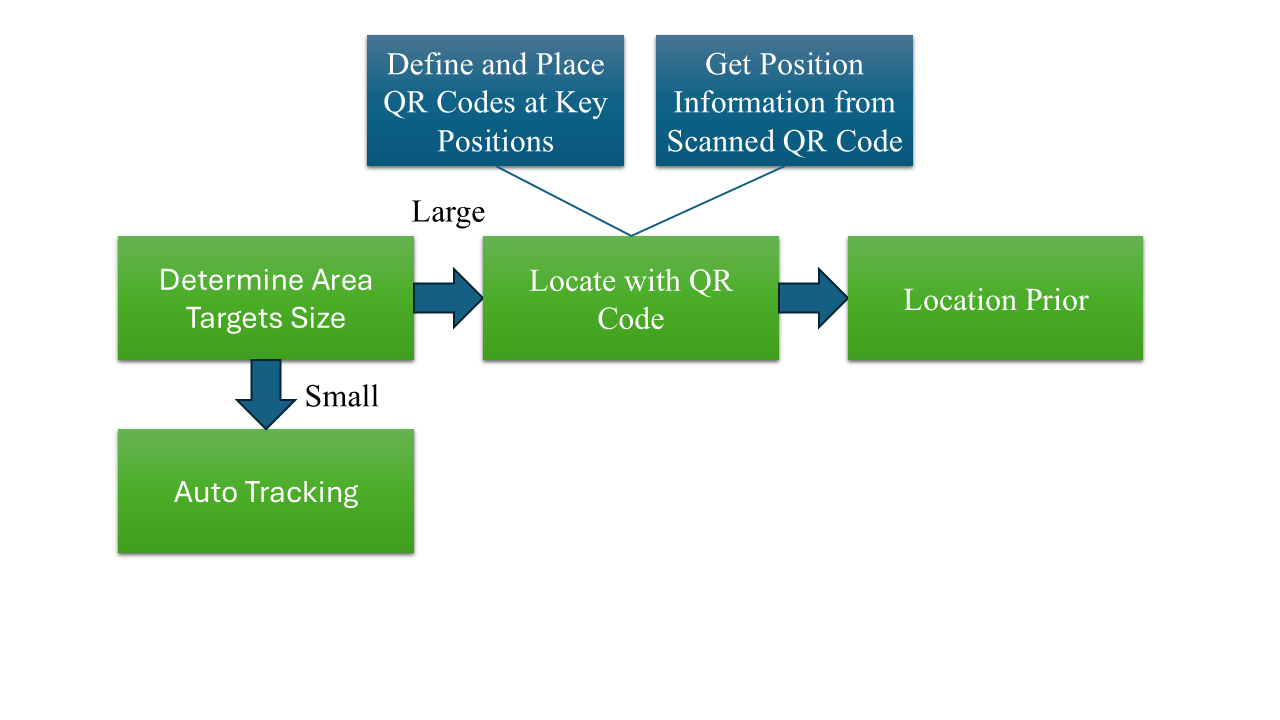
\includegraphics[scale=0.5]{content/resources/images/chap-problems-solutions/location-0.PNG}
  \caption{Workflow of Prior Location with QR Code}
  \label{fig:location-0}
\end{figure}
